% THIS IS SIGPROC-SP.TEX - VERSION 3.1
% WORKS WITH V3.2SP OF ACM_PROC_ARTICLE-SP.CLS
% APRIL 2009
%
% It is an example file showing how to use the 'acm_proc_article-sp.cls' V3.2SP
% LaTeX2e document class file for Conference Proceedings submissions.
% ----------------------------------------------------------------------------------------------------------------
% This .tex file (and associated .cls V3.2SP) *DOES NOT* produce:
%       1) The Permission Statement
%       2) The Conference (location) Info information
%       3) The Copyright Line with ACM data
%       4) Page numbering
% ---------------------------------------------------------------------------------------------------------------
% It is an example which *does* use the .bib file (from which the .bbl file
% is produced).
% REMEMBER HOWEVER: After having produced the .bbl file,
% and prior to final submission,
% you need to 'insert'  your .bbl file into your source .tex file so as to provide
% ONE 'self-contained' source file.
%
% Questions regarding SIGS should be sent to
% Adrienne Griscti ---> griscti@acm.org
%
% Questions/suggestions regarding the guidelines, .tex and .cls files, etc. to
% Gerald Murray ---> murray@hq.acm.org
%
% For tracking purposes - this is V3.1SP - APRIL 2009

\documentclass{acm_proc_article-sp}

\begin{document}

\title{ARASB: Automatic readability assessment system for Basque language}
%
% You need the command \numberofauthors to handle the 'placement
% and alignment' of the authors beneath the title.
%
% For aesthetic reasons, we recommend 'three authors at a time'
% i.e. three 'name/affiliation blocks' be placed beneath the title.
%
% NOTE: You are NOT restricted in how many 'rows' of
% "name/affiliations" may appear. We just ask that you restrict
% the number of 'columns' to three.
%
% Because of the available 'opening page real-estate'
% we ask you to refrain from putting more than six authors
% (two rows with three columns) beneath the article title.
% More than six makes the first-page appear very cluttered indeed.
%
% Use the \alignauthor commands to handle the names
% and affiliations for an 'aesthetic maximum' of six authors.
% Add names, affiliations, addresses for
% the seventh etc. author(s) as the argument for the
% \additionalauthors command.
% These 'additional authors' will be output/set for you
% without further effort on your part as the last section in
% the body of your article BEFORE References or any Appendices.

\numberofauthors{2} %  in this sample file, there are a *total*
% of EIGHT authors. SIX appear on the 'first-page' (for formatting
% reasons) and the remaining two appear in the \additionalauthors section.
%
\author{
% You can go ahead and credit any number of authors here,
% e.g. one 'row of three' or two rows (consisting of one row of three
% and a second row of one, two or three).
%
% The command \alignauthor (no curly braces needed) should
% precede each author name, affiliation/snail-mail address and
% e-mail address. Additionally, tag each line of
% affiliation/address with \affaddr, and tag the
% e-mail address with \email.
%
% 1st. author
\alignauthor
Madrazo I.\\
       \affaddr{Computer Science Department}\\
       \affaddr{Boise State University}\\
       \affaddr{1910 University Dr}\\
       \affaddr{Boise, Idaho}\\
       \email{ionmadrazo@boisestate.edu}
}


% There's nothing stopping you putting the seventh, eighth, etc.
% author on the opening page (as the 'third row') but we ask,
% for aesthetic reasons that you place these 'additional authors'
% in the \additional authors block, viz.
\additionalauthors{Additional authors: John Smith (The Th{\o}rv{\"a}ld Group,
email: {\texttt{jsmith@affiliation.org}}) and Julius P.~Kumquat
(The Kumquat Consortium, email: {\texttt{jpkumquat@consortium.net}}).}
\date{30 July 1999}
% Just remember to make sure that the TOTAL number of authors
% is the number that will appear on the first page PLUS the
% number that will appear in the \additionalauthors section.

\maketitle
\begin{abstract}
In this paper, we present a novel system for automatic readability assessment for Basque language named as ARASB. ARASB is based on a multinomial bayesian network that makes use of a set of over 4000 features generated for the task. Apart from using traditional features in the area, we present various novel features that describe characteristics of the documents, such as followability of the text or vocabulary enrichment. 

In addition, we have analyzed various methods for making good use of the inherent ordinality of the readability assessment task. The proposed system is able to predict 4 different readability levels for the input natural language documents.


\end{abstract}



\keywords{Readability assessment, Basque, Text tagging} % NOT required for Proceedings


\section{Introduction}
Readability assessment is a research area which tries to develop methods for predicting the reading difficulty of a certain text. It has been of great importance in for educational purposes even before automatic natural processing and artificial intelligence had emerged.

At that time manual formulas such as Flesh \cite{flesch1948new}, Dale-Chall \cite{chall1995readability} and Gunning FOG  \cite{albright1996readability} showed up as the most used formulas by educators for manually determining text difficulty. Most of dose formulas made use of very simple features such as, average word length or average sentence length.

\begin{figure}[h]
\begin{equation}
 Flesh =  206.835 -(1.015 * AWPS) - (84.6 * ASPW)  
\end{equation}
\caption{Flesh's readability formula ( AWPS= Average words per sentence; ASPW: average syllabes per word}
\end{figure}

Once computers and automatic natural language processing started to burst, the area changed drastically its way of developing formulas. More complex features became possible to compute by the help of computers, and supervised learning classifiers started to make appearance on the area.


Even if the main purpose of readability assessment(RA) systems is to serve as help for educator in looking for adequate texts for educator, this is not the only aim for them. RA systems have showed to be useful in areas such as book recommendation \cite{pera2014automating} for recommending books adequate for the readers capabilities or in text simplification, to determine whether or not a part of the text needs to be simplified.

 This paper is structured as follows. Section 2 provides a description of the related work of the readability assessment area. Section 3 talks about our contribution to the area. Section 4 presents a detailed description of the system. Section 5 presents the results of the experiments done. Finally, sections 6 and 7 present the conclusions and future work of this project.


\section{Related work}
In the recent years, different RA systems have been developed with high diversity regarding both languages and features. 

For English, \cite{feng2010comparison} presented a comparison of the common readability features used for English. \cite{aluisio2010readability} aimed their system for evaluating text simplification methods with a system, that made use of some more elaborated features such as ambiguity in terms. \cite{feng2009automatic} oriented their system for assessing the difficulty level of a text for people with intellectual disabilities, developing some features that were intended to detect how well a text was structured.   

For Chinese, \cite{chen2011chinese} developed a RA system only based on lexical metrics based on the TF-Idf measure. This metric in conjunction with a mutual information measure was able to determine which terms were most relevant for each of the readability levels. These terms were afterwards used to predict the level of readability for the inputs texts. However, this technique was not topic independent, as once trained for a certain topic the terms were no longer useful for other topics. Previously, \cite{collins2004language} developed a system that already tried to solve, the topic dependence problem for Chinese. This system was based on Tf-Idf too and as the authors stated, removing some top scoring words of the Tf-Idf ranking, lead the system to be more independent of the topic. Apparently, the top scoring words were highly specialized words to the topic selected for training

For Arabic, \cite{al2008towards} developed a readability assessment told based on only two features. The features were based on simple ratios based on sentence,terms and letter counts. Those, features were used with a SVM classifier in order to be able to classify text as simple or complex.

For Italian, \cite{dell2011read} presented a readability assessment system aimed for text simplification. Since the text simplification tool the authors were developing was based on sentences. The authors of this system decided,that rather than developing a system for determining text readability, their system would work at sentence level. Therefore, the text simplification tool, would have more information of which sentence needed simplification and which did not. The model generated for sentence level is shown to be generalizable to full text level, by the use of simple averages. The more complex sentences a text have, the more probabilities it have to be complex in overall.

For French,\cite{franccois2012ai} developed a readability assessment system with the foreign language learners in mind. The objective was to determine which features were more important for a foreign language learner to understand a text. In addition, they provided a metric new to the area called adjacent accuracy that tried to measure systems' performance in a more accurate and relevant. 

For Basque, for the best of our knowledge, only one system have been developed. Due to the fact that Basque is considered a minority language and shares very little similarities with the most spoken languages. Very little research have been done in the area. Therefore, currently, Errexail \cite{gonzalez2014simple} is the only system created for Basque readability assessment. This system was aimed for text simplification purposes and was developed to predict two different values, simple or complex. The aim for this was to detect which texts needed some simplification and which texts did not. The system makes use of simple features mostly based on ratios of common Natural language processing tags.


\section{Contribution}
The contribution of this paper is triple:

\begin{itemize}
\item We have developed the first readability assessment system for basque that is able to predict more than 2 readability levels.

\item We present various novel features to the area of the readability assessment

\item We present an analysis of methods that benefit from the inherent ordinality in the class values, for improving performance of the readability assessment systems.
\end{itemize}

\section{Proposed system}
Our proposed system, named as ARASB, is composed of a three step process, a general description of the pipeline can be seen in figure \ref{systempipeline}.

\begin{figure}[h]
\centering
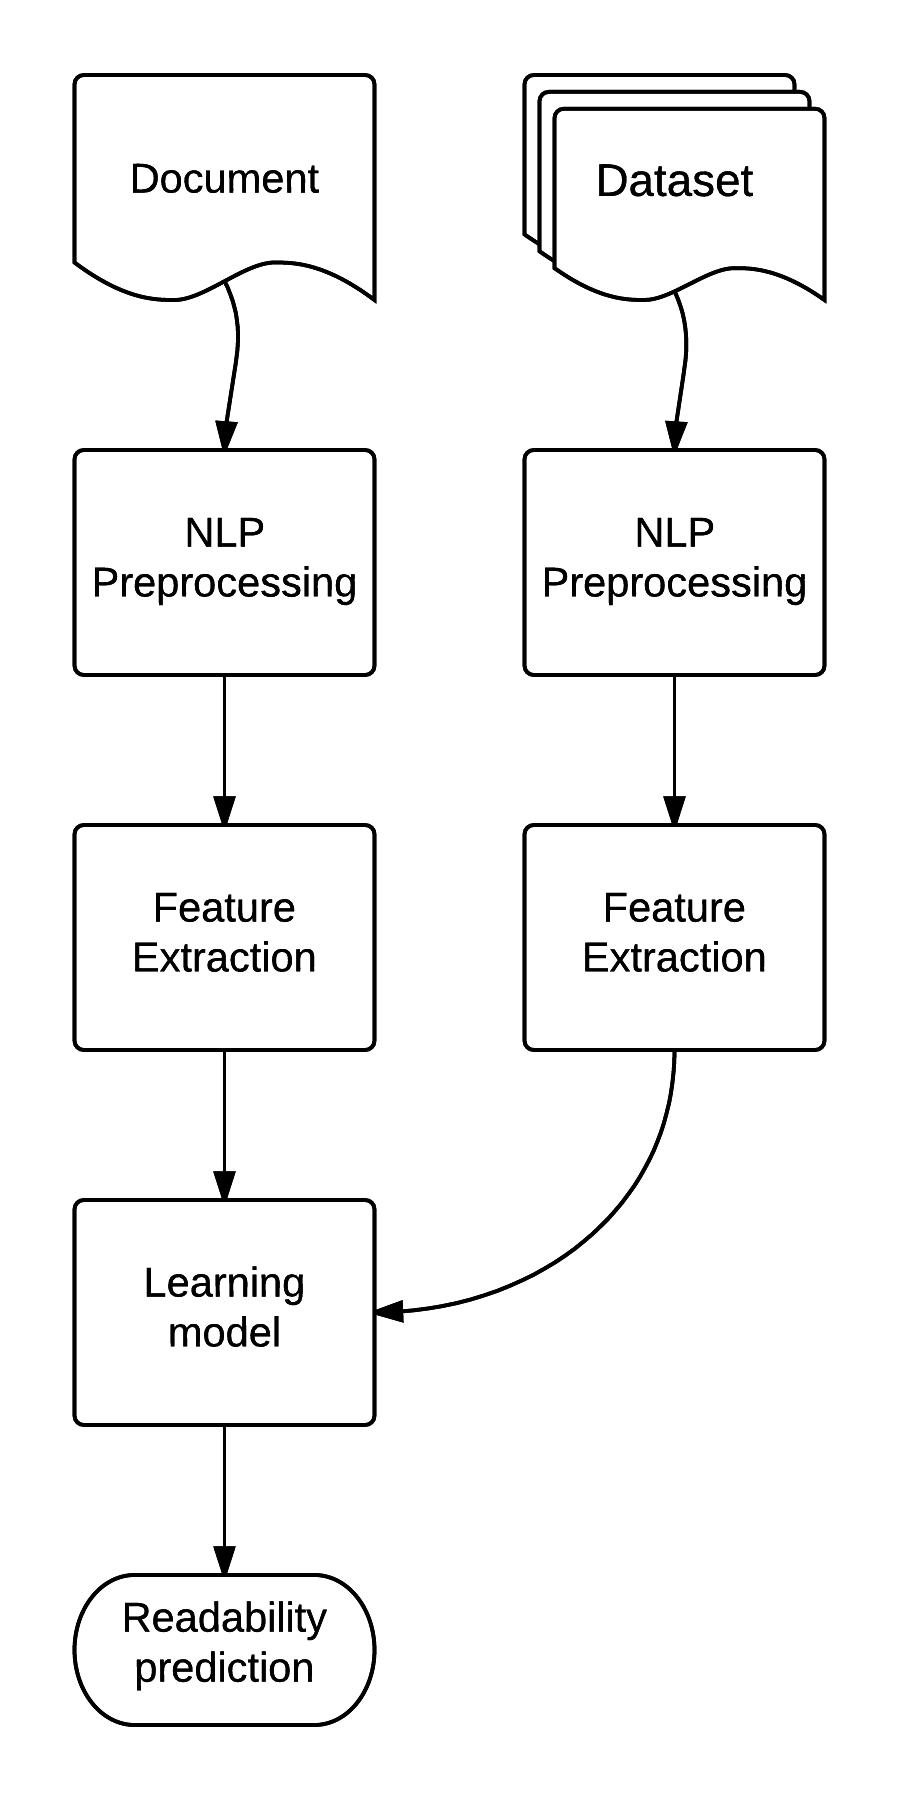
\includegraphics[width=0.4\textwidth]{systempipeline}
\caption{General system pipeline}
\label{systempipeline}
\end{figure}

 The first step consists of linguistically analyzing the plain input text. Very little features can be extracted directly from plain text, so the aim of this first step is to preprocess the plain text in order to obtain a enriched text structure.

The second step is the feature extraction phase. This step makes use of previously analyzed text in order to create more elaborated features, over the text.

The last step, is the learning/predicting step. This step makes use of the features generated in the previous step in order to create a model or predict over a previously generated model.





\subsection{Text preprocessing}
The text preprocessing phase follows a traditional well studied linguistic processing pipeline. The language tags are created in an incremental sequential way, where each analyzer  receives an input text already tagged by its predecessor and adds its part of information to it.

This way, in every step, more and more complex tags are generated over the text, creating a an structure that describes the text in various linguistic levels. All the tools used, have been specifically created for Basque language. The pipeline consists of the following analyzers:


\begin{enumerate}
\item Morpheus \cite{alegria2002robustness} for morpho-syntactic analysis .
\item Eustagger \cite{aduriz2003finite} for lemmatisation and syntactic function identification.

\item \cite{alegria2004representation} for multiword identification.

\item Ehiera \cite{alegria2004design} for Named entities recognition

\item Ixati \cite{aduriz2004cascaded} for shallow parsing.

\item Maltixa \cite{bengoetxea2010application} for sytantactic dependency parsing.

\item MuGak \cite{ aranzabe2013transforming}for detecting sentence boundaries.
\item \cite{gonzalez2013detecting} for apposition identification.

\end{enumerate}



\subsection{Features}
In this section we present the features used for the learning model. The features are ordered given their linguistic level. The most elaborated features are presented at the very end.

\subsubsection{General features}
General features consider the document as whole, and are based on quantities of words and sentences. Four features haves been defined for this group.

\begin{itemize}
\item Average number of words per sentence.
\item Average number of phrases or syntagms per sentence.
\item Average number of letters per word.
\item Percentage of terms that appear only once in the text.
\end{itemize}


\subsubsection{Lexical features}
Lexical features are features intended to describe the most basic form of a word, also known as the lemma. All the ratios are normalized against the number of words in the text.
\begin{itemize}
\item {\bf Ratios of part of speech tags}: verbs, nouns, adverbs...

\item {\bf Ratios of person tags}: Who, Who-To\_Who, Who-To\_Who-Who... (This feature is nonexistent in English)

\item {\bf Ratios of Shortenings}: acronyms, abbreviations...

\item {\bf Ratios of named entities}: person entities, place entities...

\item {\bf Ratios of modal verbs}


\end{itemize}


\subsubsection{Morphological features}
Morphological features describe the form changes suffered from lemmas. All the ratios are normalized against the number of words in the text.
\begin{itemize}
\item {\bf Ratios of case marks}: inesive, dative, acusative...


\item {\bf Ratios of aspect marks}: done or not done marks. (This feature is nonexistent in English)

\item {\bf Ratios of time marks}: past, future...
\item {\bf Ratios of mode marks}: indicative, subjunctive...

\item {\bf Ratios of ellipsis marks}: noun ellipsis, verb ellipsis...
\end{itemize}


\subsubsection{Morphosyntactic features}
Five features haves been defined for this group.

\begin{itemize}
\item Number of noun phrases per sentence.
\item Number of verb phrases per sentence.
\item Number of noun phrases per all phrases.
\item Number of verb phrases per all phrases.
\item Number of appositions per all phrases.
\end{itemize}


\subsubsection{Syntactic features}
Syntactic features are features that intend to provide information of the structure of the sentences. All the ratios are normalized against the number of words in the text.
\begin{itemize}
\item {\bf Ratios of subordinate sentences}: completive, modal, causal, final...

\item {\bf Ratios of syntactic dependences}: subject, object...



\end{itemize}

\subsubsection{Pragmatic features}
Pragmatic features provide information regarding the relations between sentences. All the ratios are normalized against the number of words in the text.
\begin{itemize}
\item {\bf Ratios of linkers}: causal, final...

\item {\bf Ratios of connectors}: conjunction, disjunction...

\end{itemize}

\subsubsection{N-gram model features}
N-gram models are a commonly used technique for natural language processing. Those models make use of of probabilities, of a term or more that one term appearing together in a text. Those probabilities are usually used as direct features for learning models.

However, these techniques, fail to achieve topic independence, due to the fact that the features themselves are composed by certain vocabulary, usually inherent to a topic.

The features we present try to follow a similar approach of n-gram models, but instead of using terms our system use probabilities of part of speech tags and syntactic dependencies.

Using this approach we create features such as, a verb followed by a verb, or a noun follows by an adjective. These features, are aimed for providing more accurate information of the structure of the sentences. Our hypothesis states, that the must be very specific structures only existent in high level texts, and some structures only existent in low level texts.

We created this type of features, with all the combinations of part of speech tags and all combinations of syntactic dependencies. Since the syntactic dependencies are modeled as a tree, the probabilities of a certain tag being the parent of another is computed, rather than the probability of a tag being followed by another. 

2-gram and 3-gram models have been used for part of speech tags and only 2-grams for syntactic dependencies.


\subsubsection{Syntactic tree depth}

A syntactic tree is a tree representation of a sentence in which every node represents a phase and the leaf nodes are the words of the sentence. In figure \ref{syntactictree} the syntactic tree of the sentence \emph{The chef cooks the soup} can be seen. The example sentence contains a noun phrase and a verb phase, which simultaneously contains another noun phase within it.

Hypothetically, the more complex the syntactic tree of a sentence is, the more complex a sentence is, and therefore, the more difficult it will be to understand. 
\begin{figure}[h]

\centering
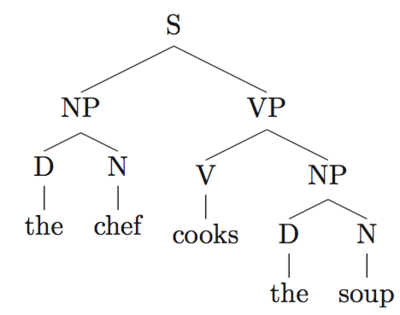
\includegraphics[width=0.45\textwidth]{syntactictree}
\caption{Example of a syntactic tree}
\label{syntactictree}
\end{figure}

To model this feature, we implemented a feature that calculates the depth of every tree in a text and and then averages it. 



\subsubsection{Vocabulary richness}
Wordnet \cite{miller1995wordnet}  is semantically structured database that is commonly used semantic analysis. The database is structured using senses that are connected between each other by sevelar semantic realations, such as synonym, anthonym or hypernym relations. For each sense, its word forms are provided. In figure \ref{wordnetHierarchy} an example of the wordnet structure can be seen. 

\begin{figure}[h]

\centering
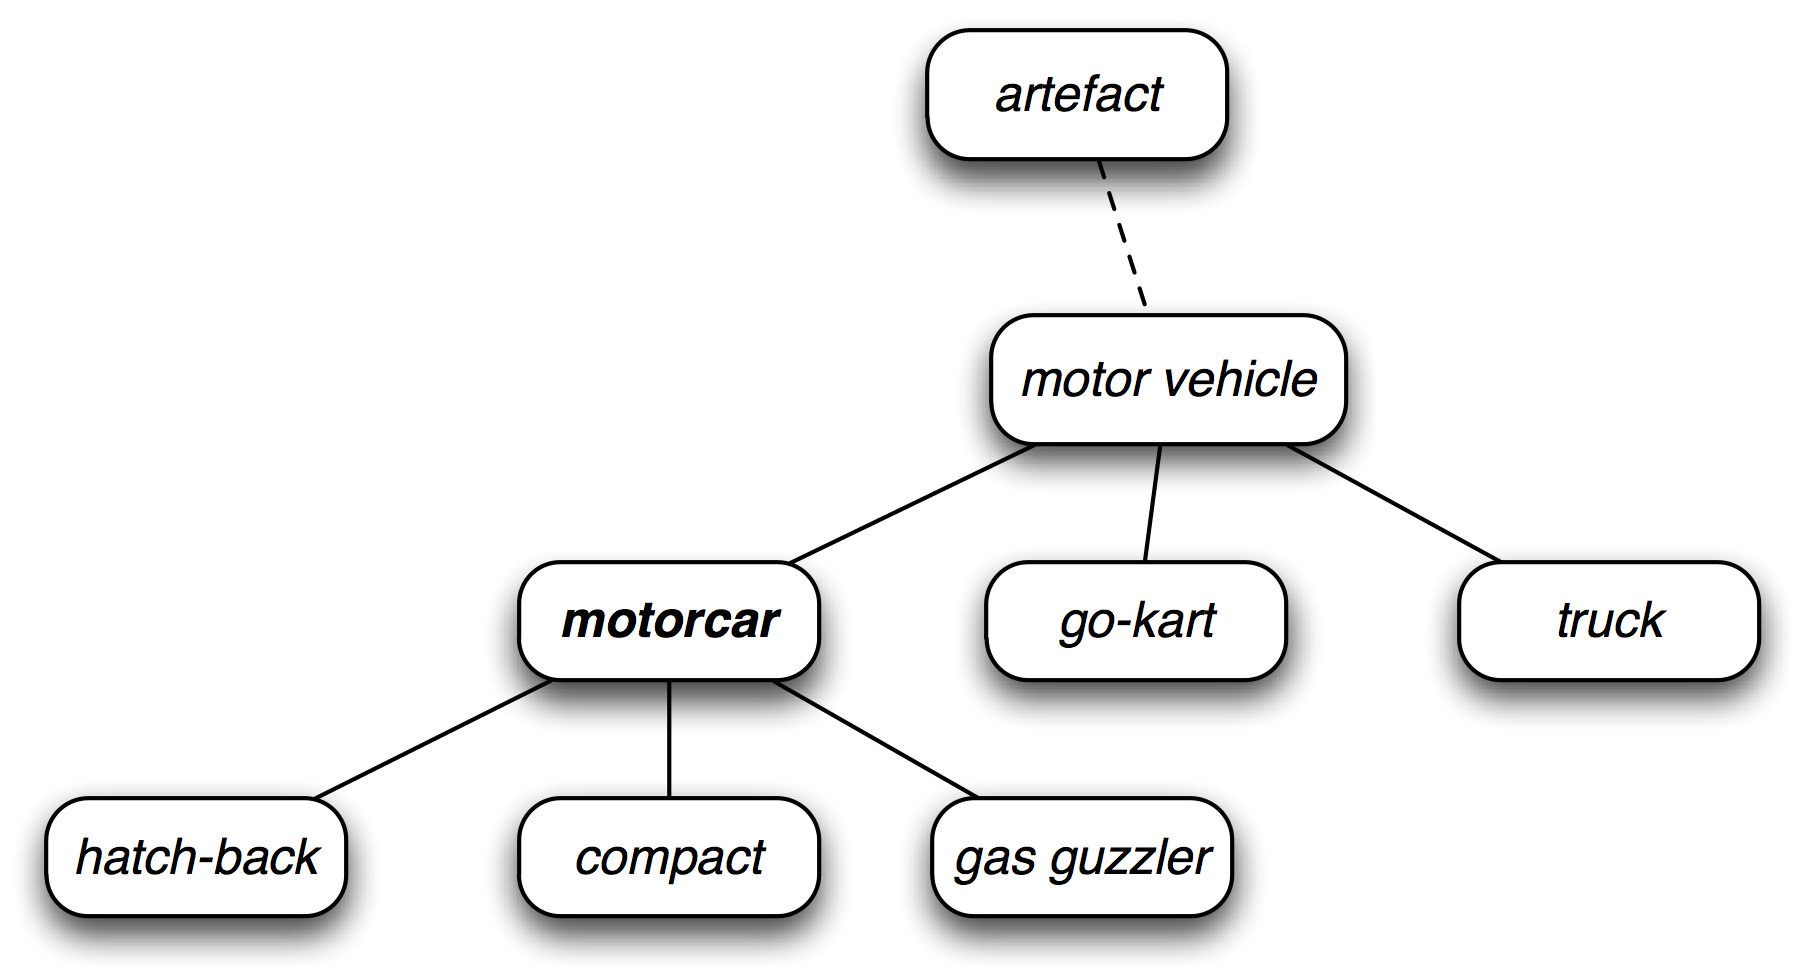
\includegraphics[width=0.45\textwidth]{wordnetHierarchy}
\caption{Example of the Wordnet structure}
\label{wordnetHierarchy}
\end{figure}

The Wordnet database contains around 120,000 different senses, and have been adapted \cite{agirre2002methodological} for multiple languages, in which Basque is included.

We have used the Wordnet database for developing a feature that describes how semantically rich is a text. Hypothetically, the more rich a text is regarding to vocabulary the more high level it should be.

For computing the measure, the first step is to extract all the senses of the text.Once, this have been done, for each sense, all its word form are retrieved from Wordnet database. Every apparition of each of those word forms is counted and stored.


Finally, in order to calculate how heterogeneous and therefore how rich is the use of vocabulary for each sense, Shannon's entropy \cite{shannon2001mathematical} is computed over the probabilities of each wordform for each sense and averaged.

By using this, measure, a sense that has have its appearance in the text by the use of only one term will receive a 0 of vocabulary richness score, and a sense that have appeared in the text in most of its possible forms will get a high vocabulary richness score.

\subsubsection{Text followability}
The aim of this feature is to measure the ease of followability of the text concepts. For this, the similarity between two sentences will be used. The more similar adjacent sentences are in a text, the softer the changes in concepts are between them and, therefore the easier it is to follow the text ideas. On the other side, the more brusque the changes between sentences are, the more concept changes are between them, and the easier is for the reader to get lost.

For computing this measure, a Latent Semantic Analysis \cite{deerwester1990indexing} \cite{landauer2013handbook} technique have been used. Latent Semantic Analysis can be used as a similarity measure between two words. LSA, works by creating a matrix of terms and documents, where a 1 is stored in each position where the term appears in that document.

\begin{table}[hbt]
 \begin{center}
 \begin{tabular}{cccccccc}
     & d1 & d2 & d3 & d4 & d5 & d6 & d7 \\ \hline
 \bf t1 & 0  & \bf 1  & 0  & 0  & 0  & \bf 1  & 0  \\
 \bf t2 & 0  & 0  & 0  & 1  & 0  & 0  & 0  \\
  t3 & 0  & 1  & 1  & 0  & 0  & 0  & 0  \\
  t4 & 0  & 0  & 0  & 0  & 0  & 0  & 0  \\
  \bf t5 & 0  & \bf 1  & 0  & 0  & 0  & \bf 1  & 0  \\
  t6 & 0  & 1  & 0  & 0  & 0  & 0  & 0  \\
  t7 & 0  & 0  & 1  & 0  & 0  & 0  & 0  \\
  t8 & 0  & 0  & 0  & 1  & 0  & 0  & 1  \\
 
 \end{tabular}
 \end{center}
 \caption{Latent Semantic Anlaysis matrix. $t_{i}$ stand for diferent terms, and $d_{i}$ stands for different documents}
 \label{tab:lsamatrizea}
\end{table}

For calculating the similarity between two term each of their vectors are compared using a cosine similarity. By this approach, having a look at the figure \ref{tab:lsamatrizea}, terms t1 and t5 are considered very similar because they co-occur in same documents, while t1 and t2 are considered completely different, because they never co-occur in a same document.

\begin{table}[h]
 \begin{center}
 \begin{tabular}{|c|c|c|c|c|c|}\hline
     & t1 & t2 & t3 & t4     & max  \\ \hline
  t5 & 0   & 0.1 & 0.5 & 0   & 0.5  \\ \hline
  t6 & 0   & 0   & 0   & 0   & 0    \\ \hline
  t7 & 0.2 & 0.4 & 0.9 & 0   & 0.9  \\ \hline
  t8 & 0.3 & 0.4 & 0.9 & 1   & 1    \\ \hline
     &     &     &     &     & avg:0.6    \\ \hline
   
 
 \end{tabular}
 \end{center}
 \caption{Computing followability. t1, t2, t3 and t4 represent one sentence and t5, t6, t7 and t8 represent another one. Each cell value represents the LSA score between it row term and its column term.}
 \label{tab:jarraitasunsemantikoa}
\end{table}

For computing the followability between two sentences, the procedure in figure \ref{tab:jarraitasunsemantikoa} is followed. Each term in the first sentence is matched with LSA against each term in the second sentence, calculating the maximum LSA scores for each of the terms in the first sentences. Those maximum values are averaged in order to compute a sentence to sentence LSA similarity. This same procedure is followed for each adjacent sentence pain in the text and averaged.


For training the LSA model, a set of a month of daily articles of a Basque newspaper called \emph{Egunkaria} have been used. 



\subsection{Learning models}
Apart from the commonly used supervised learning algorithms, various new to the area algorithms have been used for developing ARASB. In this section we present the algorithms used, and the main motivation for using them.
\subsubsection{CFS Feature Subset Selection}
Given that the developed feature set is considerably large(over 4000 features), feature selection has been a important task of the learning task. The algorithm we have used for feature subset selection is the one presented by \cite{hall1998practical}.

This algorithm makes use of a greedy space search algorithm that uses a correlation based heuristic. The heuristic this algorithm uses, tends to prefer subsets with features with high correlation regarding the class to predict, and with low correlation between each other. This way, this algorithm tries to find a near to optimal subset that reduces the number of features by avoiding redundant information.


\subsubsection{Ordinal Classification}
The automatic readability assessment task has a inherent ordinarily in the class values that has not usually taken into account for learning purposes. Methods exist that make use of this ordinality in order to improve performance of the classifiers. ARASB makes use of the algorithm presented in \cite{frank2001simple}. This algorithm works by creating multiple binary classifiers in a hierarchical way to take profit of the ordinality of the class values.


\subsubsection{Cost Sensitive Learning}
Cost sensitive learning \cite{ling2010cost}, is the set of methods that try to introduce a sense of cost in the learning process. E.g.: For a classifier that tries to predict breast cancer, has not the same cost a false positive, and a false negative.  Making a false negative error has a considerably higher cost than a false positive, because the life of a person is in risk in the first case. 

A similar thing happens in readability assessment. If a RA system makes an error in predicting the readability level from 1 to 10 for an instance that has a readability value of 1, the cost is not the same if the predicted value is 2 or if the predicted value is 10. The error would be considered larger, when the system predicted a 10.

Therefore, cost sensitive learning have been used in ARASB with the purpose of minimizing the errors magnitude, with the trade-off of sightly lowering the the general accuracy of the system.

\section{Experiment}
In this section we present the experiment carried for analyzing the system. Firstly, we present the dataset used for the experiment. Secondly, we show an analysis of the features developed for the system. Finally, a general analysis of ARASB is shown.

\subsection{Dataset}
Finding a readability leveled dataset for Basque is not a easy task. The education contents for basque are very reduced and most of them are not publicly available. 

The dataset we have used for the experiment have been extracted from an online basque learning web page called Ikasbil\footnote{http://www.ikasbil.net/}. This web page contains leveled reading exercises aimed for Basque learners. The leveling is done ussin the European framework of languages, which consists of 6 levels, named as, A1, A2, B1, B2, C1 and C2.  
\begin{table}[h]
 \begin{center}
 \begin{tabular}{|c|c|c|c|c|c|}\hline
  A1 & A2 & B1 & B2 & C1 & C2\\ \hline
  1 & 24 & 481 & 2497 & 748 & 39\\ \hline
 
 \end{tabular}
 \end{center}
 \caption{Number of texts per level of readability.}
 \label{tab:ikasbilTestuKopuruak}
\end{table}

The number of documents for each level can be seen in table \ref{tab:ikasbilTestuKopuruak}. The number of text for each level are not homogeneous, and levels A1, A2 and C2 have a very low quantity of texts.

Given that no other dataset was available for the experiment, a decision to discard levels A1 and A2 have been made and level C2 have been complimented with texts from a high level science divulgation web page, called Zientzia \footnote{http://zientzia.eus/}. Those text are of enough complexity to be considered of C2 level.

With addition of the documents from Zientzia, a dataset of 1200 documents have been created, with 300 documents for each level of readability, B1, B2, C1 and C2.



\subsection{Feature analysis}
 Two different analysis have been carried for features. Firstly, an overall analysis is presented with the aim of finding the most important features regarding the whole system. Secondly, an analysis of features regarding their importance for each readability level is presented.
\subsubsection{General Analysis}
In figure \ref{tab:top10orokorra} the top 10 features with highest information gain can be seen. Some of the novel features introduced in this paper seem to have a high importance regarding predicting readability. Features such as n-gram ratios or the more elaborated methods such as vocabulary richness are present in the top 10 of the feature ranking.

\begin{table}
 \begin{center}
 \begin{tabular}{|c|c|}\hline
  {\bf Information Gain} & { \bf Feature } \\ \hline
 0.27807 & Ratio of modal verbs \\ \hline
 0.20147 & Linker + Linker 2-gram ratio \\ \hline
 0.20142 & Verb + Verb + Verb 3-gram ratio \\ \hline
 0.19855 & Vocabulary richness \\ \hline
 0.19542 & Syntactic Tree depth \\ \hline
 0.1927 & Ratio of verb phases \\ \hline
 0.18055 & Linker + Noun 2-gram \\ \hline
 0.17576 & Verb + Verb 2-gram \\ \hline
 0.17535 & Average length of words \\ \hline
 0.16693 & Linker(emend) ratio \\ \hline
 
 \end{tabular}
 \end{center}
 \caption{Top 10 features, ordered by information gain. Whole system.}
 \label{tab:top10orokorra}
\end{table}


 
\begin{figure}[h]

\centering
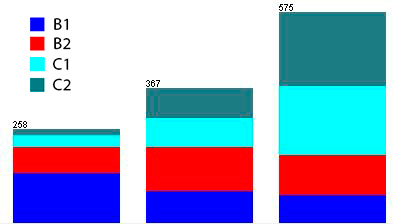
\includegraphics[width=0.45\textwidth]{disc_sakonera_orokorra}
\caption{Discretization for syntactic tree depth feature}
\label{disc_sakonera_orokorra}
\end{figure}

In figure \ref{disc_sakonera_orokorra}, it can be seen that when values of the tree depth feature are high (x axis), the presence of high level documents is higher that when its values are low. This shows that the hypothesis we made when developing this feature was correct. Same happens with other developed features.

\begin{table}
 \begin{center}
 \begin{tabular}{|c|c|}\hline
  {\bf Group of Features} & { \bf Avg. Info. gain } \\ \hline
 	Lexical &  0.076 \\ \hline
    Morphologic & 0.068 \\ \hline
    Morfosyntactic & 0.097 \\ \hline
    Syntactic & 0.083 \\ \hline
    Pragmatic & 0.093 \\ \hline
 
 
 \end{tabular}
 \end{center}
 \caption{Grouped features ordered by information gain}
 \label{tab:IGmultzokatuaOrokorra}
\end{table}
In the figure \ref{tab:IGmultzokatuaOrokorra} the features can be seen grouped by its linguistic level. Morfosysntactic level seems to be the most relevant set of features for determining text readability, followed by pragmatic level. 


\begin{table*}
 \begin{center}
 \begin{tabular}{|c|c|c|c|c|c|}\hline

 {\bf Class }     &{\bf TP rate}   & {\bf FP rate} & {\bf Accuracy (Adjacent accuracy)} & {\bf Recall}  &  {\bf F-Measure}   \\ \hline
 {\bf B1   }       &      0,533     &  0,140        &  0,559 (0,853)          &  0,533        &   0,546            \\ \hline
 {\bf B2   }       &      0,430     &  0,188        &  0,433 (0,999)          &  0,430        &   0,431            \\ \hline
 {\bf C1   }       &      0,750     &  0,184        &  0,575 (0,973)          &  0,750        &   0,651            \\ \hline
 {\bf C2   }       &      0,723     &  0,009        &  0,964 (0,978)          &  0,723        &   0,827            \\ \hline

  
 \end{tabular}
 \end{center}
 \caption{Multinomial naive bayes, detailed results}
 \label{tab:aukeratuaestatistikak}
\end{table*} 
\subsubsection{Per level Analysis}
The same analysis have been done on a per level basis. For each readability level a binary class have been created that takes as positive example a document form that class and as negative all other documents. Same information gain analysis have been done over those new set, getting diverse results regarding the top 10 features.


For level B1, the top 10 highest information gain features are mostly syntactic dependency based ones. Level B2, seem to be determined by the presence of subordinate sentences, commonly learned at that level. For level C1, the features that have most information gain seem to be related to n-grams, especially related to some certain complex structures such as verb + verb + verb. This level have a light presence of linker features too. Finally, level C2, is strongly influenced by linker related features, 5 out of 10 top features are related to linker presence.

\subsection{System analysis}
For analysis the system as a whole, the data have been divided into two sets, training (2 out of 3 parts) and test. The training dataset have been used in the algorithm selecting process, using a 10-fold cross validation procedure. Finally, once all the decisions for the system were made, the system have been tested against the test dataset. 

For the test purposes, the feature set that have been used is a subset generated by the CFS feature subset algorithm, which consists of 56 features.

\subsubsection{Selecting learning algorithm}
The system have been tested with different learning models to determine which one fit the best to it. In table \ref{tab:sailkapenalgoritmoakasmatze} a comparison of the tested learning algorithms can be seen. It can be seen that, the three bayesian algorithms and the logistic regression algorithms outperform the algorithms based on nearest neighbor and trees. However, all 4 algorithms are statistically similar in terms of accuracy. Just for the reason of selecting one, for the next experiments, the multinomial naive bayes network algorithm have been chosen. 

\begin{table}
 \begin{center}
 \begin{tabular}{|c|c|c|}\hline
  {\bf Algorithm} & {\bf Accuracy} & {\bf T-test} \\ \hline
   Gaussian Bayes net.             & 57.33 $\pm$ 2.02 & Base \\ \hline
   Multinomial N. bayes net. & 61.69 $\pm$ 2.48 & S.E. \\ \hline
   Bayes net. 3 parents. & 60.29 $\pm$ 2.07 & S.E. \\ \hline
   C4.5                       & 51.99 $\pm$ 2.52 & S.W. \\ \hline
   1NN                       & 51.81 $\pm$ 2.05 & S.W. \\ \hline
   5NN                       & 56.00 $\pm$ 1.02 & S.W. \\ \hline
   Log. regression       & 58.90 $\pm$ 1.83 & S.E. \\ \hline
  
 \end{tabular}
 \end{center}
 \caption{Comparison of learning algorithms. S.E: Statistically Equal: S.W: Statistically Worse. p<0.05}
 \label{tab:sailkapenalgoritmoakasmatze}
\end{table}

In table \ref{tab:aukeratuaestatistikak}, a more detailed information of the performance of the selected algorithm can be seen. Even if the comparison is not fully reliable, the accuracy result shown are at the level of other state of the art systems.
 

\subsubsection{Ordinal Classification}

In table \ref{tab:ordinalttest} the results of the comparison between using or not using the ordinal classification previously mentioned can be seen. The use of ordinal algorithms increases the performance in a statistically significant way, validation our hypothesis that such an algorithm would benefit a readability assessment system.
\begin{table}
 \begin{center}
 \begin{tabular}{|c|c|}\hline
	        Naive Bayes   & Naive Bayes + ordinal classification    \\ \hline
 				60.87 $\pm$ 3.83  &   62.52 $\pm$ 4.17 \\ \hline
 \end{tabular}
 \end{center}
 \caption{Ordinal classification with naive bayes vs. naive bayes}
 \label{tab:ordinalttest}
\end{table} 

\subsubsection{Cost Sensitive Analysis}
The cost matrix for the cost sensitive algorithm can be seen in table \ref{tab:kostuMatrizea}. The cost function we used to test our system increases the error cost exponentially, for every unit of distance from the real value.
\begin{table}
 \begin{center}
 \begin{tabular}{|c|c|c|c|c|}\hline

     & {\bf B1} &  {\bf B2} &  {\bf C1} & {\bf C2 }  \\ \hline
{\bf B1}	  &  0   &  1 & 10    &   1000       \\ \hline
{\bf B2}   &       1 & 0  &  1   &   10     \\ \hline
{\bf C1	}   &      10  &  1 &  0  &  1    \\ \hline
{\bf C2	}     &    1000  &  10 &   1  & 0      \\ \hline
  
 \end{tabular}
 \end{center}
 \caption{Cost matrix}
 \label{tab:kostuMatrizea}
\end{table}  

The use of the cost sensitive function, decreases the general performance significantly regarding usual accuracy, as it was expected. However, this method increases significantly the adjacent accuracy of the system. Those results can be seen on tables \ref{tab:costsensitivettest} and \ref{tab:costsensitivettestadjacent}.

\begin{table}
 \begin{center}
 \begin{tabular}{|c|c|}\hline
	        Naive Bayes   & Naive Bayes + cost sensitive    \\ \hline
 				60.87 $\pm$ 3.83  &   58.79 $\pm$ 4.52 \\ \hline
 \end{tabular}
 \end{center}
 \caption{Cost sensitive vs. Naive Bayes }
 \label{tab:costsensitivettest}
\end{table} 


\begin{table}
 \begin{center}
 \begin{tabular}{|c|c|}\hline
	        Naive Bayes   & Naive Bayes + cost sensitive    \\ \hline
 				95.07 $\pm$ 1.24  &   97.34 $\pm$ 1.33 \\ \hline
 \end{tabular}
 \end{center}
 \caption{Cost sensitive vs. Naive Bayes (adjacent accuracy)}
 \label{tab:costsensitivettestadjacent}
\end{table} 

\subsubsection{Final test}
After doing different test, the final systems is the composition of CFS feature subset selection, multinomial Naive Bayes, ordinal classification and cost sensitive learning method. The results of the final ARASB system against the test dataset can be seen on table \ref{tab:aukeratuaestatistikakTest}. All the results seem to be similar, with a slight decrease, to the ones obtained using the training set with cross validation.




\begin{table*}
 \begin{center}
 \begin{tabular}{|c|c|c|c|c|c|}\hline

 {\bf Class }     &{\bf TP rate}   & {\bf FP rate} & {\bf Accuracy} & {\bf Recall}  &  {\bf F-Measure}   \\ \hline
 {\bf B1   }       &      0,463    &  0,104  &    0,633   &     0,463   &   0,535             \\ \hline
 {\bf B2   }       &      0,390    &  0,226    &  0,400    &    0,390    &  0,395              \\ \hline
 {\bf C1   }       &      0,659   &   0,330    &  0,435    &    0,659    &  0,524              \\ \hline
 {\bf C2   }       &      0,583    &  0,008    &  0,933     &   0,583   &   0,718           \\ \hline
{\bf Batazbestekoa } &    0,517  &    0,186  &    0,562  &      0,517   &   0,523             \\ \hline
  
 \end{tabular}
 \end{center}
 \caption{Final system, detailed test results}
 \label{tab:aukeratuaestatistikakTest}
\end{table*}  

\section{Conclusions}
In this paper we presented ARASB, a tool that is able to predict the readability level of a text with a state of the art accuracy. The system is able to predict, over 4 levels of readability, which doubles the quantity of readability levels compared to its predecessor, ErreXail.

The novel features created for the system have shown high prediction ability regarding the class values.

We have introduced two novel approachs to the area of readability assessment, which make use of the inherent ordinality in the class values with success. 



\section{Future work}


As future work, we would like to test our project with a bigger and fuller dataset that contained the missing A1 and A2 readability levels.

We would like to do research in other methods for measuring the followability of the texts, methods based on concept maps that have already been used with success in other areas.

Another interesting experiment would be to take a parallel dataset in two different languages, and do an analysis of the features that affect each language. This way, we could have a better idea of what is important in which language and probably why.







%\end{document}  % This is where a 'short' article might terminate



%
% The following two commands are all you need in the
% initial runs of your .tex file to
% produce the bibliography for the citations in your paper.
\nocite{*}
\bibliographystyle{apalike}
\bibliography{sigproc}  % sigproc.bib is the name of the Bibliography in this case
% You must have a proper ".bib" file
%  and remember to run:
% latex bibtex latex latex
% to resolve all references
%
% ACM needs 'a single self-contained file'!
%
%APPENDICES are optional
%\balancecolumns

\end{document}
